% Chapter 1

\chapter{Introducción general} % Main chapter title

\label{Chapter1} % For referencing the chapter elsewhere, use \ref{Chapter1} 
\label{IntroGeneral}
En este capítulo se realiza una breve introducción de los elementos externos que interactúan con el sistema con la finalidad de brindar un marco de comprensión general antes de realizar un abordaje específico. También se explica el alcance y objetivos del presente trabajo.

%----------------------------------------------------------------------------------------

% Define some commands to keep the formatting separated from the content 
\newcommand{\keyword}[1]{\textbf{#1}}
\newcommand{\tabhead}[1]{\textbf{#1}}
\newcommand{\code}[1]{\texttt{#1}}
\newcommand{\file}[1]{\texttt{\bfseries#1}}
\newcommand{\option}[1]{\texttt{\itshape#1}}
\newcommand{\grados}{$^{\circ}$}

%----------------------------------------------------------------------------------------
%----------------------------------------------------------------------------------------
\section{Descargas parciales}
Según IEEE

(Guide for the Measurement of Partial Discharges in AC Electric Machinery)
\enquote{Una DP (descarga parcial) es una descarga eléctrica que cortocircuita parcialmente el material aislante ubicado entre dos conductores. Cuando la tensión excede cierto valor crítico, se produce una ionización gaseosa transitoria en el sistema aislante, a dicha ionización se la denomina DP} \citep{IEEE:citation}

Una descarga parcial es un fenómeno de disrupción eléctrica. Se caracteriza por ser un pulso de corriente de alta frecuencia el cual se produce en el seno de un sistema aislante de una máquina o equipo eléctrico de potencia de media o alta tensión como consecuencia de la presencia de  oclusiones gaseosas, impurezas aristas aguzadas u otras anomalıas que distorsionan la distribución de las lineas de campo eléctrico, figura \ref{fig:basicoDp}.

\begin{figure}[ht]
	\centering
	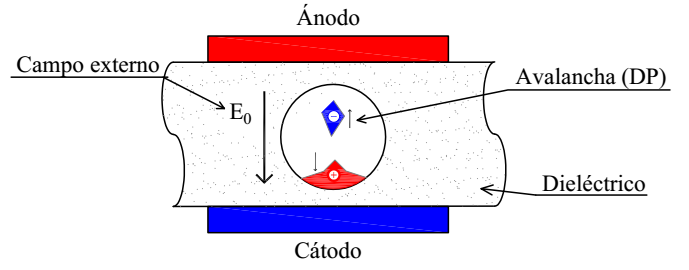
\includegraphics[width=\textwidth]{./Figures/basicoDp.png}
	\caption{Esquema básico de DP en el interior de un aislante.}
	\label{fig:basicoDp}
\end{figure}

La ocurrencia de este fenómeno provoca un deterioro del sistema aislante. Dependiendo del medio en el que este fenómeno se manifiesta y cuál sea la causa que lo origina, el deterioro del sistema es acumulativo.

\subsection{Medidores de descargas parciales}
La técnica eléctrica más utilizada para medir una DP, se basa en registrar las corrientes que se producen en el seno del medio aislante mediante la utilización de sensores inductivos pasivos de alta frecuencia conectados en las derivaciones a tierra de los equipos que se desean ensayar.
Cuando la DP se produce en el interior del sistema aislante, las corrientes que circulan hacia tierra pasan a través de un sensor inductivo; induciendo una fuerza electromotriz proporcional a la carga involucrada, figura \ref{fig:dpEjemplo}.

\begin{figure}[ht]
	\centering
	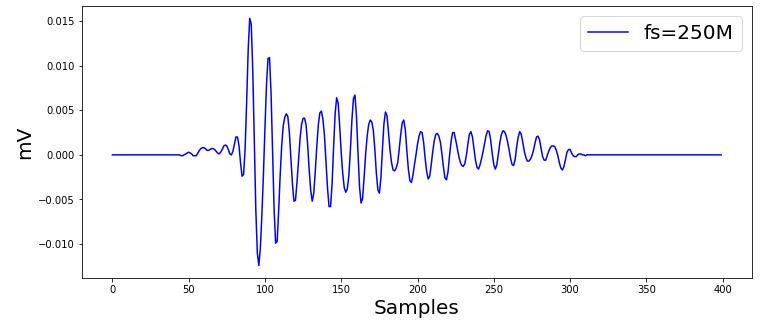
\includegraphics[width=\textwidth]{./Figures/dpEjemplo.png}
	\caption{Forma de onda de una descarga parcial capturada por un HFCT (high frequency current transformer).}
	\label{fig:dpEjemplo}
\end{figure}

Las DP registradas son utilizadas dentro de un sistema de referencias, en su eje de ordenadas se representa la máxima amplitud del pulso y en el eje de abscisas el momento angular correspondiente de la senoide de referencia de 50 Hz. Por medio de la superposición de múltiples eventos sobre un mismo periodo de 50 Hz se conforma lo que se conoce en la literatura especializada como Diagrama de Magnitud - Fase o Patrón de DP, figura \ref{fig:patronEjemplo}.

\begin{figure}[!ht]
	\centering
	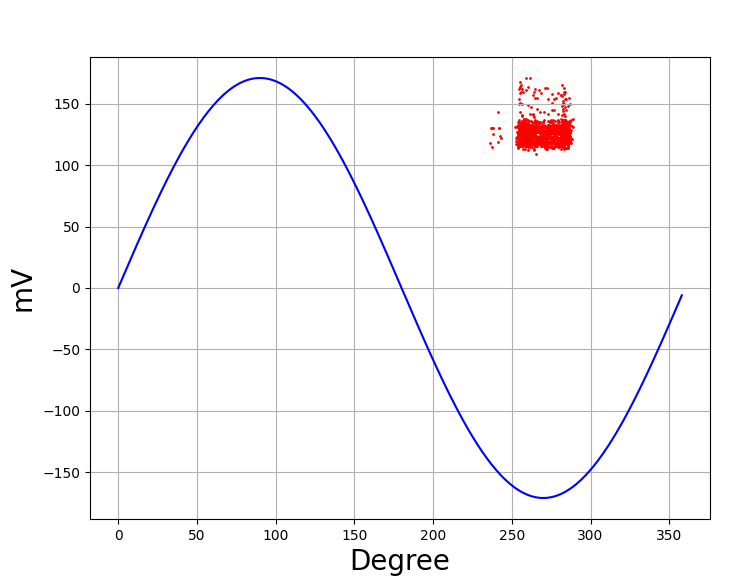
\includegraphics[width=100mm]{./Figures/patronEjemplo.png}
	\caption{Patrón de descargas parciales.}
	\label{fig:patronEjemplo}
\end{figure}

Los patrones de descargas parciales permiten identificar, por medio de su interpretación, diferentes tipos de DP \citep{Gulski:citation}, y mediante la identificación del tipo es posible emitir un diagnóstico y conocer el grado de severidad de un falla, ya que distintos tipos de DP tienen asociados distintos riesgos \citep{Cavallini:citation}.

Sensor inductivo
Los transformadores de corriente de alta frecuencia (HFCT), figura \ref{fig:hfct}, son sensores inductivos adecuados para adquisiciones de DP. Estos se instalan abrazando la pantalla del cable de descarga a tierra sobre el que se desea medir la descarga parcial. 

\begin{figure}[ht]
	\centering
	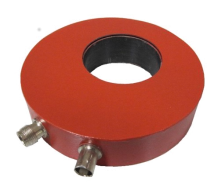
\includegraphics[width=70mm]{./Figures/hfct.png}
	\caption{HFCT de la empresa BlueBox.}
	\label{fig:hfct}
\end{figure}

\section{Estado del arte}
Actualmente existen equipos de medición de descargas parciales fabricados por empresas extranjeras como TechImp, PD Power Diagnostix, Omnicrom. Si bien esta gama de equipos abarca un amplio rango de características, ninguno proporciona una herramienta considerada de bajo costo para nuestro país, que permita a cooperativas o medianas empresas acceder a este herramienta de diagnóstico. Al mismo tiempo, este equipo proporciona una herramienta de base para implementar algoritmos propios para procesamiento over the edge; características que no tienen los actuales equipos en el mercado, los cuales operan con herramientas de procesamiento muy anticuadas.

Entre los equipos existentes se pueden mencionar los siguientes por su similitud.


TechImp Falcon
\begin{itemize}
\item Solución “económica” para monitoreo constante de descargas parciales.
\item Adquisición automática y generación del patrón de descargas parciales.
\item Separación de las diferentes actividades de descargas.
\item Ancho de banda 30 Mhz resolución 12 bits.
\item Conexión ethernet.
\end{itemize}

\begin{figure}[h!]
	\centering
	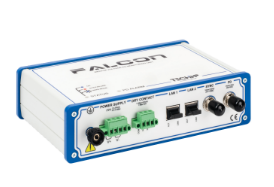
\includegraphics[width=80mm]{./Figures/arte1.png}
	\caption{Equipo Falcon de Techimp.}
	\label{fig:arte1}
\end{figure}


\vspace{10mm}
PD Power Diagnostix ICMmonitor
\begin{itemize}
\item Creación del patrón y display para visualización in-situ.
\item Analizador de espectro.
\item Posibilidad de monitoreo remoto.
\item Conexión TCP.
\end{itemize}

\begin{figure}[h!]
	\centering
	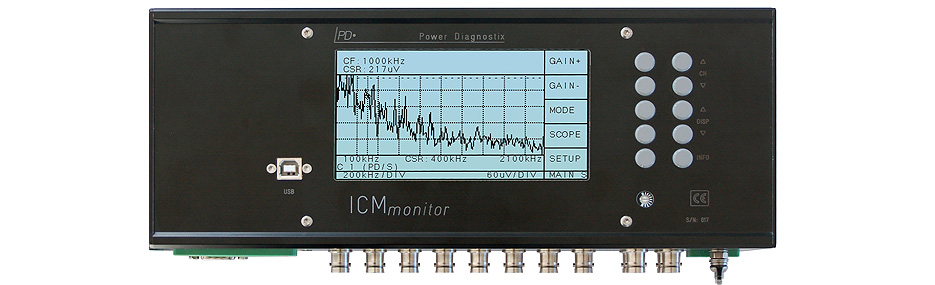
\includegraphics[width=90mm]{./Figures/arte2.png}
	\caption{Equipo ICMmonitor de Pdix.}
	\label{fig:arte2}
\end{figure}


Omicrom MPD600
\begin{itemize}
\item Medicion y analisis de descargas
\item Permite grabar, analizar y mostrar las señales.
\end{itemize}

\begin{figure}[h!]
	\centering
	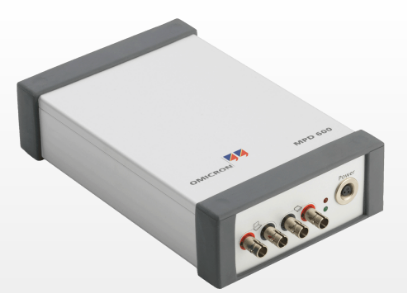
\includegraphics[width=80mm]{./Figures/arte3.png}
	\caption{MPD600 de Omnicrom.}
	\label{fig:arte3}
\end{figure}

\section{Objetivos y alcance}
\subsection{Objetivos}
El objetivo de este trabajo fue generar un equipo adquisidor de descargas parciales de calidad, de bajo costo y de producción nacional. A su vez, se buscó generar las bases para obtener un equipo abierto con capacidad de hacer procesamiento over the edge. 

\subsection{Alcance}
El alcance del trabajo incluyó:
\begin{itemize}
\item El desarrollo del prototipo del producto.
\item El desarrollo del firmware.
\item El diseño del circuito esquemático.
\item Confección de un manual de uso.
\item Pruebas de validación y verificación.
\end{itemize}

